\documentclass{article}
\usepackage{xeCJK}
\usepackage[utf8]{inputenc}
\usepackage{graphicx}
\usepackage{soul}
\usepackage{caption}
\usepackage[utf8]{inputenc}
\usepackage{amsmath}
\usepackage[dvipsnames]{xcolor}
\DeclareMathOperator*{\argmax}{arg\,max}
\DeclareMathOperator*{\argmin}{arg\,min}

\title{Hidden Markov models: definition and properties}
\author{Yun-Hsiang Chan}
\date{May 2021}

\begin{document}

\maketitle

\section*{I. The basics of HMM}
\subsection*{1.1 Definition and notation}

\textbf{Hidden Markov Model $\{X_t: t \in N$\}} is a particular kind of dependent mixture model. With $X^{(t)}$ and $C^{(t)}$ representing the histories from time $1$ to $t$, one can summarize the simplest model of this kind by: 

$$Pr(C_t | C^{(t-1)}) = Pr(C_t | C_{t-1}), t = 2, 3, ...$$
$$Pr(X_t | X^{(t-1)}, C^{(t)}) = Pr(X_t | C_t), t \in \mathcal{N}$$
\\
The model consists of two parts: \\
1. An unobserved 'parameter process' $\{C_t: t = 1, 2, ...\}$ satisfying the Markov property. \\
2. The 'state dependent process' $\{X_t: t = 1, 2, ...\}$, in which the distribution of $X_t$ depends only on the current state $C_t$ and not on previous states or observation. \\
\\
See figure 1 for the structure. \\
\begin{figure}
    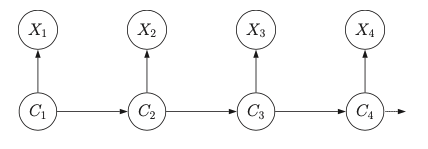
\includegraphics[width = 10cm]{Screen Shot 2021-06-04 at 4.58.33 PM.png}
    \caption{HMM structure}
\end{figure}
\\
We call Markov chain $\{C_t\}$ has $m$ states, we call $\{X_t\}$ an $m$-state HMM. \\
\\
We now introduce some notation which will cover both discrete and continous-valued observations. In the case of discrete observations we define, for $i = 1, 2, ..., m$
$$p_i(x) = Pr(X_t = x | C_t = i)$$
\\
That is, $p_i$ is the probability mass function of $X_t$ if the Markov Chain is in state $i$ at time $t$. The continuous case is trated similarly: there we define $p_i$ to be the probability density function of $X_t$ associated with state $i$. We refer to the $m$ distributions $p_i$ as the \textbf{state-dependent distributions} of the model. 

\subsection*{1.2 Marginal distributions}
We shall often need the marginal distribution of $X_t$ and also higher-order marginal distributions, such as that of $(X_t, X_{t+k})$. We shall derive the results for the case in which the Markov chain is homogeneous but not necessarily stationary, and then give them also for the special case in which the Markov chain is stationary. \\
\\
\textbf{- Univariate distributions} \\
For discrete-valued observations $X_t$, defining $u_i(t) = Pr(C_t = i)$ for $t = 1, ..., T$, we have: 
\begin{align}
    Pr(X_t = x) & = \sum_{i=1}^m Pr(C_t = i) Pr(X_t = x | C_t = i) \\
    & = \sum_{i=1}^m u_i(t)p_i(x)
\end{align}
In matrix notation: 
\begin{align}
    Pr(X_t = x) & = (u_1(t), ..., u_m(t)) \begin{pmatrix} p_1(x) & & 0 \\ & ... & \\ & ... & \\ 0 & & p_m(x) \end{pmatrix}  \\
    & = u(t) P(x) 1'
\end{align}
where $P(x)$ is defined as the diagonal matrix with ith diagonal element $p_i(x)$. It follows that $u(t) = u(1) \Gamma^{t-1}$, and hence that 
$$Pr(X_t = x) = u(1) \Gamma^{t-1} P(x) 1'$$
\\
The equation holds if the Markov chain is merely homogeneous, and not necessarily stationary. If, as we shall often assume, the Markov chain is stationary, with stationary distribution $\delta$, then the result is simpler: in that case $\delta \Gamma^{t-1} = \delta$ for all $t \in N$, and so 
$$Pr(X_t = x) = \delta P(x) 1'$$
\\
\textbf{- Bivariate distribution}
In any directed graphical model, the joint distribution of a set of random variables $V_i$ is given by 
$$Pr(V_1, V_2, ..., V_n) = \Pi_{i=1}^n Pr(V_i | pa(V_i))$$
where $pa(V_i)$ denotes the set of all parents of $V_i$ in the set $V_1, V_2, ..., V_n$ \\
\\
For example, $X_t, X_{t+k}, C_t, C_{t+k}$, $C_t$ has no parents, $pa(X_t) = \{C_t\}$, $pa(C_{t+k}) = \{C_t\}$ and $pa(X_{t+k}) = \{C_{t+k}\}$, and
$$Pr(X_t, X_{t+k}, C_t, C_{t+k}) = Pr(C_t) Pr(X_t|C_t) Pr(C_{t+k} | C_t) Pr(X_{t+k} | C_{t+k})$$
\begin{align}
    Pr(X_t = v, X_{t+k} = w) & = \sum_{i=1}^m \sum_{j=1}^m Pr(X_t = v, X_{t+K} = w, C_t = i, C_{t+k} = j) \\
    & = \sum_{i=1}^m \sum_{j=1}^m Pr(C_t = i) p_i(v) Pr(C_{t+k} = j | C_t = i) p_j(w) \\
    & = \sum_{i=1}^m \sum_{j=1}^m u_i(t) p_i(v) \gamma_{ij}(k) p_j(w) \\
    & = u(t) P(v) \Gamma^k P(w) 1'
\end{align}
\\
If the Markov chain is stationary, this reduces to
$$Pr(X_t = v, X_{t+k} = w) = \delta P(v) \Gamma^k P(w) 1'$$
\\
Similarly, for the higher-order marginal distributions, in the stationary case, 
$$Pr(X_t = v, X_{t+k} = w, X_{t+k+l} = z) = \delta P(v) \Gamma^k P(w) \Gamma^l P(z) 1'$$

\subsection*{1.3 Moments}
$$E(X_t) = \sum_{i=1}^m E(X_t | C_t = i) = \sum_{i=1}^m u_i(t) E(X_t | C_t = i)$$
In the stationary case, it reduces to 
$$E(X_t) = \sum_{i=1}^m \delta_i E(X_t | C_t = i)$$
And for $E(g(X_t))$
$$E(g(X_t)) = \sum_{i=1}^m \delta_i E(g(X_t) | C_t = i)$$
$$E(g(X_t, X_{t+k})) = \sum_{i, j = 1}^m E(g(X_t, X_{t+k}) | C_t = i, C_{t+k} = j) \delta_i \gamma_{ij}(k)$$
\\
Also, we can factorize $g(X_t, X_{t+k}) = g_1(X_t, g_2(X_{t+k}))$, so, the equation will become
$$E(g(X_t, X_{t+k})) = \sum_{i, j = 1} E(g_1(X_t | C_t = i)) E(g_2 (X_{t+k}) | C_{t+k} = j) \delta_i \gamma_{ij}(k)$$
\\
These expressions enable us to find covariances and correlations. 

\section*{II. The likelihood}
The aim of this section is to develop a convenient formula for the likelihood $L_T$ of $T$ consecutive observations $x_1, x_2, ..., x_T$ assumed to be generated by an $m$-state HMM.

\subsection*{2.1 The likelihood of a two-state Bernoulli-HMM}

See the example in the textbook.

\subsection*{2.2 The likelihood in general}
Suppose we there is an observation sequence $x_1, x_2, ..., x_T$ genreated by such a model. We seek the probability $L_T$ of observing that sequence, as calculated under an $m$-state HMM which has initial distribution $\delta$ and $\Gamma$ for the Markov chain, and state dependent probability function $p_i$. \\
\\
\textbf{Proposition 1}
$$L_T = \delta P(x_1) \Gamma P(x_2) \Gamma P(x_3) ... \Gamma P(x_T) 1'$$
If $\delta$, the distribution of $C_1$, is the stationary distribution of the Markov chain, then in addition
$$L_T = \delta \Gamma P(x_1) \Gamma P(x_2) ... \Gamma P(x_T) 1'$$
Proof: See Figure 2
\begin{figure}
    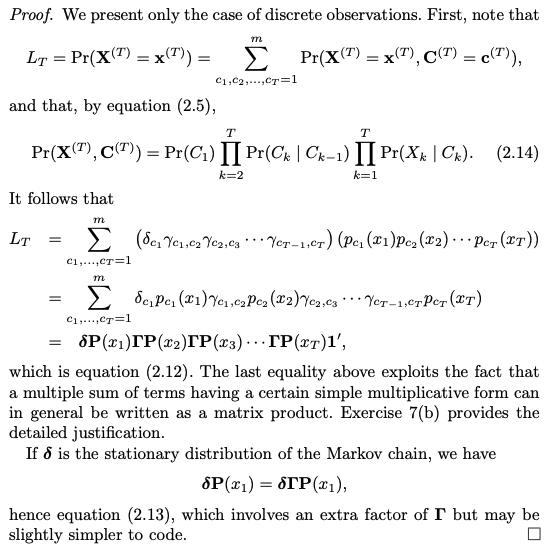
\includegraphics[width = 12cm]{proof.png}
    \caption{Proof of Proposition 1}
\end{figure}
\\
\\
The simple but cruial consequence of the matrix expression for the likelihood is the 'forward' algorithm for recursive computation of the likelihood. The recursive nature of the likelihood evaluation via the formulas is computationally much more efficient than brute-force summation over all possible state sequences. \\
\\
To state the forward algorithm, we define $\alpha_t$, for $t =1, 2, ... T$ by 
$$\alpha_t = \delta P(x_1) \Gamma P(x_2) \Gamma P(x_3) ... \Gamma P(x_t) = \delta P(x_1) \Pi_{s=2}^t \Gamma P(x_s)$$
It follows immediately from this definition that
$$L_T = \alpha_T 1' \text{, and } \alpha_t = \alpha_{t-1}\Gamma P(x_t) \text{, for } t \geq 2$$
\\
Accordingly, we can conventiently set out as follows the computations involved in the likelihood formula (1):
$$\alpha_1 = \delta P(x_1)$$
$$\alpha_t = \alpha_{t-1} \Gamma P(x_t) \text{, for } t = 2, 3, ..., T$$
$$L_T = \alpha_T 1'$$
\\
If the Markov chain is stationary, then 
$$\alpha_0 = \delta$$
$$\alpha_t = \alpha_{t-1} \Gamma P(x_t) \text{, for } t = 1, 2, 3, ..., T$$
$$L_T = \alpha_T 1'$$
\\
The elements of $\alpha_t$ are usually referred to as \textbf{forward probabilities}.

\subsection*{2.3 HMMs are not Markov processes}

HMMs do not in general satisfy the Markov property, i.e. 
$$Pr(X_t | X_{t-1}) \neq Pr(X_t | X_{t-1}, X_{t-2}, ... ,X_1)$$
This can be established via some simple counterexamples.

\subsection*{2.4 The likelihood when data are missing}
In a time series context it is potentially awkward if some of the data are missing. In the case of hidden Markov time series models, however, the adjustment that needs to be made to the ilkelihood computation if data are missing turns out to be a simple one. \\
\\
Suppose that one has observations $x_1, x_2, x_4, x_7, x_8, ..., x_T$ of an HMM, but $x_3, x_5$ and $x_6$ are missing, then the likelihood is 
\begin{align}
Pr(X_1 = x_1, X_2 = x_2, X_4 = x_4, ..., X_T = x_T) & = \sum \delta_{c_1} \gamma_{c_1, c_2} \gamma_{c_2, c_4}(2) \gamma_{c_4, c_7} (3) .... \\
& \times p_{c_1}(x_1) p_{c_2}(x_2) p_{c_4}(x_4)... \\
& = \delta P(x_1) \Gamma P(x_2) \Gamma^2 P(x_4) \Gamma^3 P(x_7) ... 1'
\end{align}
\\
In general, in the expression for the likelihood the diagonal matrices $P(x_t)$ corresponding to missing observations $x_t$ are replaced by the identity matrix; that is, the corresponding state-dependent probabilities $p_i(x_t)$ are replaced by $1$ for all states $i$.

\subsection*{2.5 The likelihood when observations are interval-censored}
For interval-censored distributions, suppose $a \leq x_t \leq b$, we replace the diagonal matrices $P(x_t)$ in the likelihood expression by the $m \times m$ diagonal matrix of which the ith diagonal element is $Pr(a \leq X_t \leq b | C_t = i)$





\end{document}